\section{Exploración Espacial}\label{espacial}

La ruta más expedita para salir de la pobreza es el desarrollo humano. Para impulsarlo debe haber acceso a servicios de salud y educación de buena calidad. Si Colombia quiere tener pros-peridad y justicia social, requiere atender la equidad entre sus zonas rurales y urbanas, entre sus regiones, entre grupos étnicos y entre hombres y mujeres en aspectos como el acceso a la educación, la propiedad de la tierra y la distribución del ingreso.




Nuevos estudios sugieren que el estrés de ser pobre tiene una peligrosa influencia en la salud. Cuando se comparan los estados socioeconómicos altos y bajos, el riesgo de algunas enfermedades es diez veces mayor. Las personas de estrato socioeconómico bajo tienen dramáticamente más riesgo de enfermar y expectativa de vida más corta.


\begin{Schunk}
\begin{Soutput}
  Group.1       IDH  cabeLog restoLog
1       1 0.7944545 13.54188 12.74991
2       2 0.8575000 15.28062 13.57715
3       3 0.7890000 11.42861 11.21085
\end{Soutput}
\end{Schunk}


\begin{figure}[h]
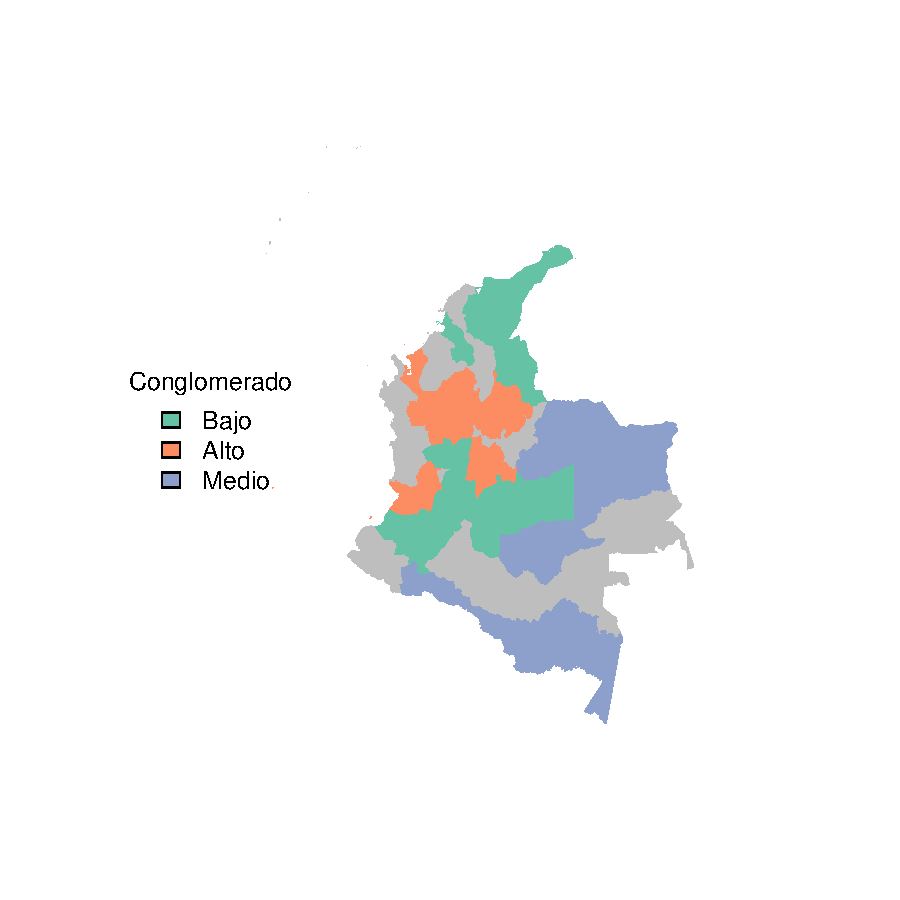
\includegraphics{Espacial-plotMap1}
\caption{Paises conglomerados segun sus indicadores sociopolíticos}\label{clustmap}
\end{figure}

Se requieren 50,000 millones de dólares, según la ONU que pueden obtenerse de cualquiera de estas fuentes: si los ricos pagaran 0.2 porciento del valor de su patrimonio, si por cada tonelada de dióxido de carbono que se vierta a la atmósfera se pagara 10 dólares, si a los 210,000 millones de dólares de las transacciones financieras diarias, se aplicara una tasa de 0.005 porciento, si las multinacionales dieran 1 porciento de sus beneficios, si de las ventas legales de armas se dedicara 10 porciento de ayuda al desarrollo. Es decir, hay capacidad y recursos suficientes en el mundo para erradicar el hambre y la pobreza y promover el desarrollo económico sustentable con justicia social. Mientras, de los 6 mil millones de habitantes del planeta 40 porcciento viven con menos de dos dólares al día, sólo 10 porciento vive bien, con altos ingresos anuales per cápita y utilizando los beneficios culturales y tecnológicos alcanzados por la humanidad. Es un escándalo que teniendo los medios para erradicarla, el hambre tenga que esperar y mate a 24,000 personas por día y 11 niños por minuto.

\endinput
